\label{chap:prospective}

Though stars are, overall, generally considered to be well-understood, a number of open problems remain in asteroseismology and, more widely, the field of stellar astrophysics as a whole. 
At a basic level, we currently are unable to predict stellar radii from first principles. 
This is due to the fact that we use time-independent one-dimensional theories of convection in evolutionary models---approximations which are controlled by free parameters. 
Properly modelling convection in stellar interiors seems to be among the biggest goals in modern theoretical stellar astrophysics. 
Furthermore, for similar reasons, we generally fail to predict pulsation frequencies of stars, even after making post-hoc corrections for near-surface effects. 

Along similar lines, one of the most basic facts about stars (and astronomical bodies in general) is that they rotate. 
Yet canonical stellar modelling often neglects the effects of rotation, and other similarly `obvious' phenomena such as magnetic fields. 
The very long-term future of research into stars may feature fully 3D magnetohydrodynamical stellar modelling, or even a full treatment of every individual particle that make up the star; however, it is clear that we are far away from that point. 
%Along similar lines, canonical stellar modelling neglects the effects of rotation and magnetic fields.
%This also gives rise to surface effects, which is a nuisance in practically every asteroseismic investigation. 
%Solving convection seems to be the most important  
%Here I will state what I perceive to be some prospects for these areas of research. 
%we can't even predict stellar radii!!!
%The surface term 
%The nature of convective energy transport 
%Fully 3D magnetohydrodynamical stellar modelling 
%Rotation and magnetism 

In terms of the continuation of the research presented in this thesis, there are a few avenues in particular that I intend to explore in the coming months and years: 
\begin{description}
    \setlength{\itemindent}{0pt}
    \item[Structure inversions of more stars.]
    The next step is to apply the technique developed in Chapter~\ref{chap:inversion} to as many stars as possible. 
    This will allow us to determine whether the theory of stellar evolution produces models with the correct interior structures. 
    
    Figures~\ref{fig:phy} and \ref{fig:phy2} show structure inversions for $20$~stars from the \emph{Kepler} LEGACY sample \citep{2017ApJ...835..172L}. 
    The reference models have been constructed under four different assumptions of input physics: with/without diffusion, and with/without convective core overshooting. 
    While some stars show broad agreement throughout their interior with evolutionary models (e.g., KIC~$5184732$), most of the models disagree substantially with the interior structure of the stars. 
    Furthermore, there seems to be no set of input physics considered here that repairs the differences. 
    This indicates that important ingredients may be missing from canonical models of stellar interiors, such as mixing induced by internal rotation. 

%\afterpage{
\begin{figure}
    \centering
    \adjustbox{trim=0cm 1.4cm 0cm 0cm, clip}{%
        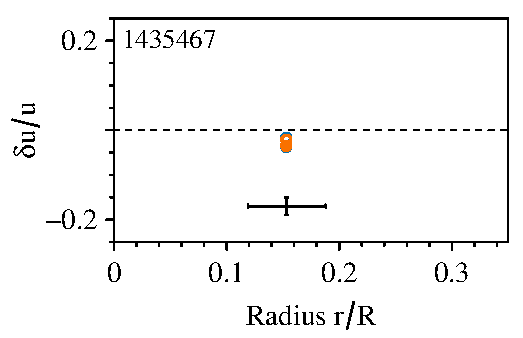
\includegraphics[width=0.55\textwidth]{ch1_introduction/figs/prospective/inversion/1435467.pdf}%
    }%
    \adjustbox{trim=1.6cm 1.4cm 0cm 0cm, clip}{%
        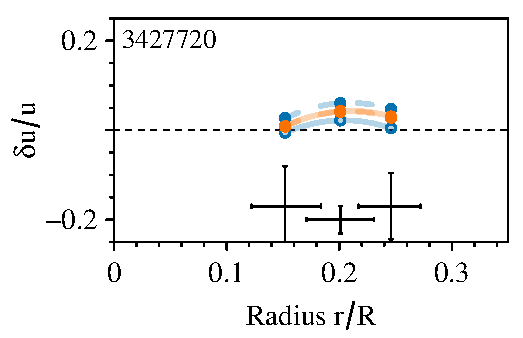
\includegraphics[width=0.55\textwidth]{ch1_introduction/figs/prospective/inversion/3427720.pdf}%
    }\\%
    \adjustbox{trim=0cm 1.4cm 0cm 0cm, clip}{%
        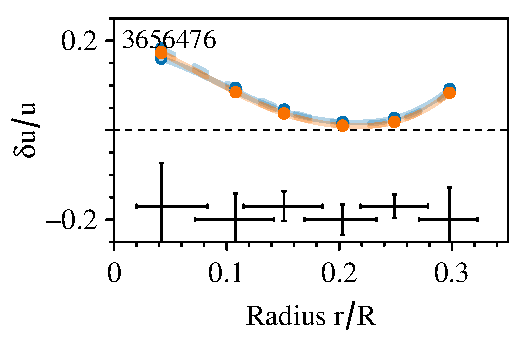
\includegraphics[width=0.55\textwidth]{ch1_introduction/figs/prospective/inversion/3656476.pdf}%
    }%
    \adjustbox{trim=1.6cm 1.4cm 0cm 0cm, clip}{%
        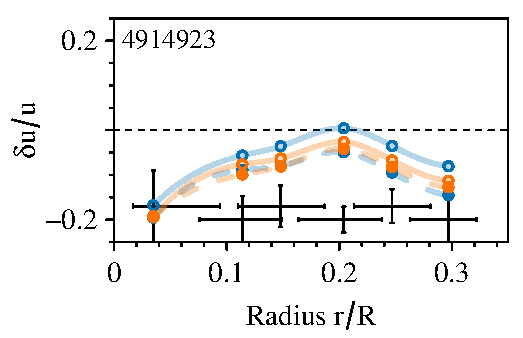
\includegraphics[width=0.55\textwidth]{ch1_introduction/figs/prospective/inversion/4914923.pdf}%
    }\\%
    \adjustbox{trim=0cm 1.4cm 0cm 0cm, clip}{%
        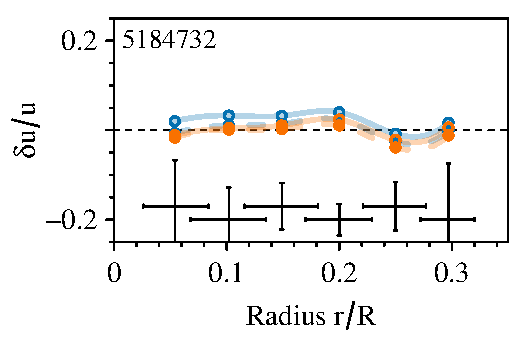
\includegraphics[width=0.55\textwidth]{ch1_introduction/figs/prospective/inversion/5184732.pdf}%
    }%
    \adjustbox{trim=1.6cm 1.4cm 0cm 0cm, clip}{%
        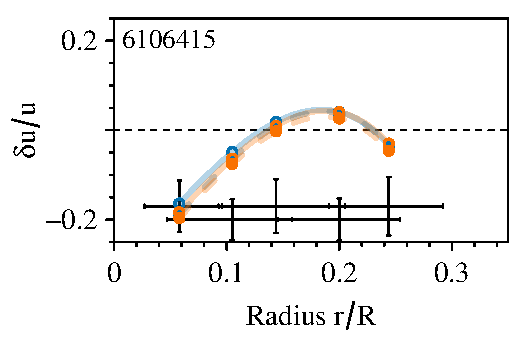
\includegraphics[width=0.55\textwidth]{ch1_introduction/figs/prospective/inversion/6106415.pdf}%
    }\\%
    \adjustbox{trim=0cm 1.4cm 0cm 0cm, clip}{%
        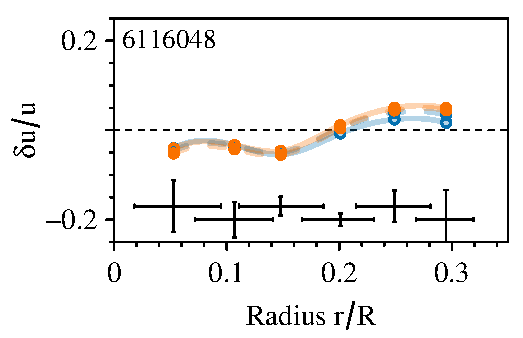
\includegraphics[width=0.55\textwidth]{ch1_introduction/figs/prospective/inversion/6116048.pdf}%
    }%
    \adjustbox{trim=1.6cm 1.4cm 0cm 0cm, clip}{%
        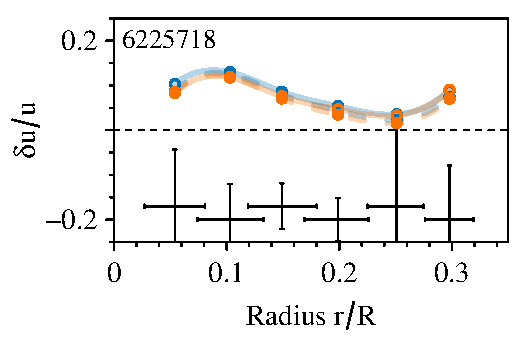
\includegraphics[width=0.55\textwidth]{ch1_introduction/figs/prospective/inversion/6225718.pdf}%
    }\\%
    \adjustbox{trim=0cm 0cm 0cm 0cm, clip}{%
        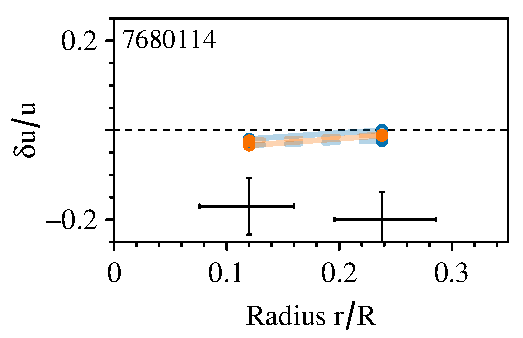
\includegraphics[width=0.55\textwidth]{ch1_introduction/figs/prospective/inversion/7680114.pdf}%
    }%
    \adjustbox{trim=1.6cm 0cm 0cm 0cm, clip}{%
        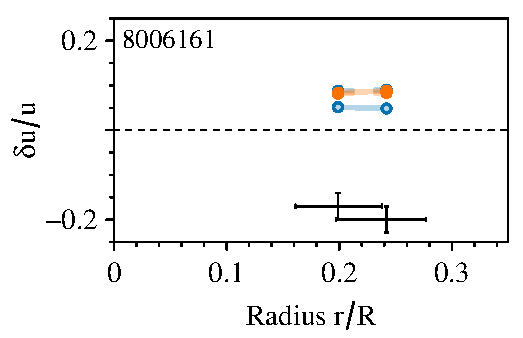
\includegraphics[width=0.55\textwidth]{ch1_introduction/figs/prospective/inversion/8006161.pdf}%
    }%
    \caption[Inversion Zoo]{(Continued in Figure~\ref{fig:phy2}.) \label{fig:phy}}
\end{figure}
\begin{figure}
    \centering
    \adjustbox{trim=0cm 1.4cm 0cm 0cm, clip}{%
        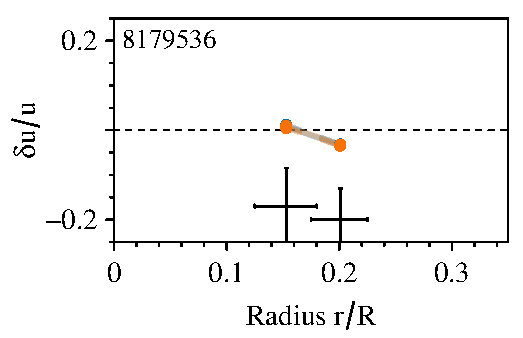
\includegraphics[width=0.55\textwidth]{ch1_introduction/figs/prospective/inversion/8179536.pdf}%
    }%
    \adjustbox{trim=1.6cm 1.4cm 0cm 0cm, clip}{%
        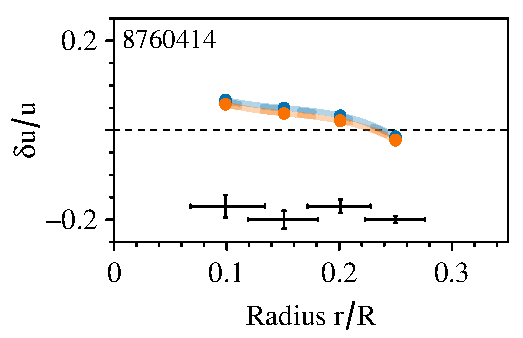
\includegraphics[width=0.55\textwidth]{ch1_introduction/figs/prospective/inversion/8760414.pdf}%
    }\\%
    \adjustbox{trim=0cm 1.4cm 0cm 0cm, clip}{%
        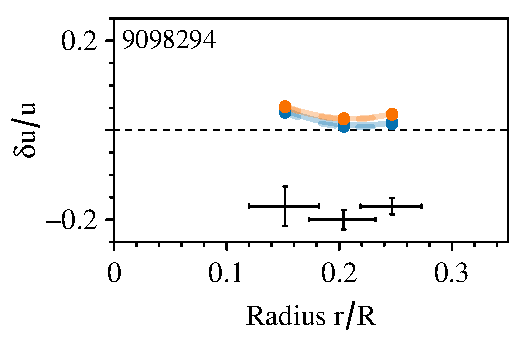
\includegraphics[width=0.55\textwidth]{ch1_introduction/figs/prospective/inversion/9098294.pdf}%
    }%
    \adjustbox{trim=1.6cm 1.4cm 0cm 0cm, clip}{%
        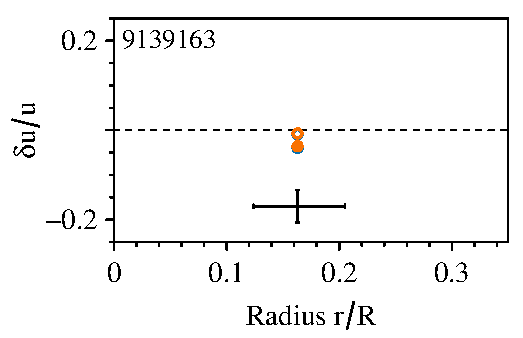
\includegraphics[width=0.55\textwidth]{ch1_introduction/figs/prospective/inversion/9139163.pdf}%
    }\\%
    \adjustbox{trim=0cm 1.4cm 0cm 0cm, clip}{%
        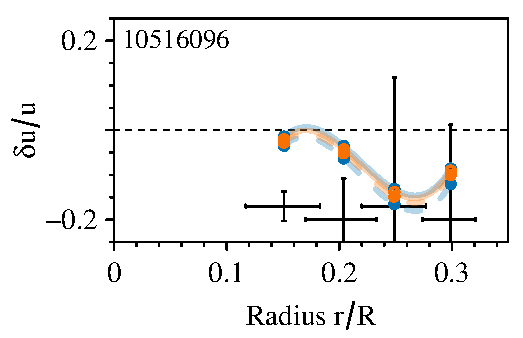
\includegraphics[width=0.55\textwidth]{ch1_introduction/figs/prospective/inversion/10516096.pdf}%
    }%
    \adjustbox{trim=1.6cm 1.4cm 0cm 0cm, clip}{%
        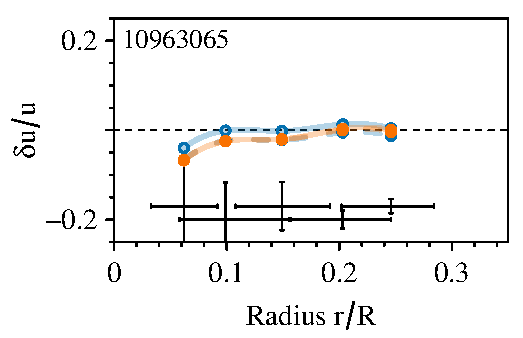
\includegraphics[width=0.55\textwidth]{ch1_introduction/figs/prospective/inversion/10963065.pdf}%
    }\\%
    \adjustbox{trim=0cm 1.4cm 0cm 0cm, clip}{%
        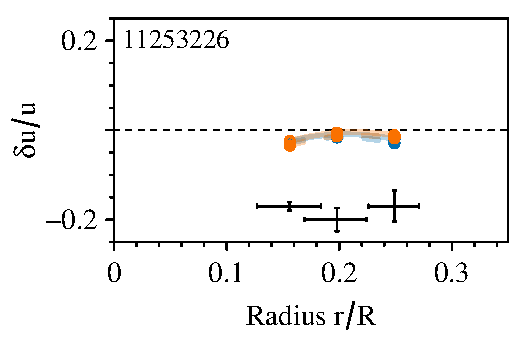
\includegraphics[width=0.55\textwidth]{ch1_introduction/figs/prospective/inversion/11253226.pdf}%
    }%
    \adjustbox{trim=1.6cm 1.4cm 0cm 0cm, clip}{%
        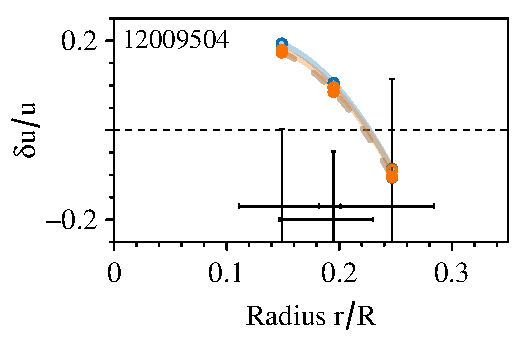
\includegraphics[width=0.55\textwidth]{ch1_introduction/figs/prospective/inversion/12009504.pdf}%
    }\\%
    \adjustbox{trim=0cm 0cm 0cm 0cm, clip}{%
        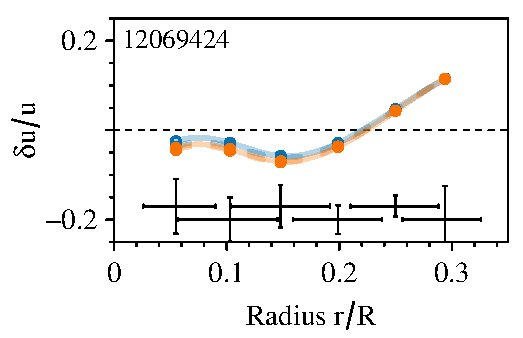
\includegraphics[width=0.55\textwidth]{ch1_introduction/figs/prospective/inversion/12069424.pdf}%
    }%
    \adjustbox{trim=1.6cm 0cm 0cm 0cm, clip}{%
        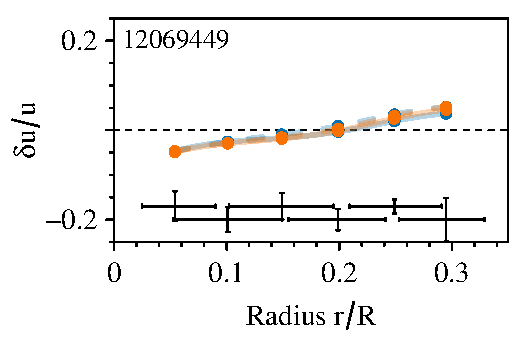
\includegraphics[width=0.55\textwidth]{ch1_introduction/figs/prospective/inversion/12069449.pdf}%
    }%
    \caption[]{(Caption on other page.)
    \label{fig:phy2}}
\end{figure}
%}
\begin{figure}
    \contcaption{Core sound-speed profiles of LEGACY stars compared against stellar models constructed with different physics inputs: with/without diffusion (orange/blue, respectively) and with/without overshooting (filled/open points, respectively). 
    The quantity $\delta u/u$ is the relative difference in the isothermal speed of sound between the model and the star at that location in the stellar interior. 
    The uncertainties of the inversion results and the widths of the corresponding averaging kernels are shown as error bars in the bottom of each panel, and are vertically offset from one another for visibility. }
\end{figure}
    
    This work is soon to be submitted to the Astrophysical Journal. 
    
    
    \item[Evolution inversions of evolved stars.] 
    There have been at least an order of magnitude more detections of solar-like oscillations in evolved stars such as red giants than in main-sequence stars. 
    When combined with kinematic information, determining the ages and chemical compositions of a large number of red giant stars will allow us to reconstruct the history of the Galaxy's development.
    
    In Chapter~\ref{chap:intro} I showed the future evolution of the Sun up through to core helium exhaustion. 
    Current ongoing work is the application of the techniques developed in Chapters~\ref{chap:ML} and \ref{chap:statistical} to these later stages of evolution.  
    
    
    \item[Structure inversions of evolved stars.]
    In this thesis, I analyzed main-sequence solar-like oscillators. 
    After stars leave the main sequence, the $p$-modes in their envelopes mix with the $g$-modes in their deep interiors to give rise to mixed modes of oscillation. 
    Figure~\ref{fig:kernel-evol} shows the evolution of the kernel function for an ${\ell=1}$ mixed mode throughout the sub-giant phase of evolution. 
    After obtaining suitable reference models, for example using the technique mentioned in the previous point, I will invert mixed mode frequencies to determine the core structures of sub-giant and eventually red-giant stars. 
    This presents the exciting prospect for potentially learning more about the deep core structure of another star than we know about our own Sun. 

%\begin{landscape}
\begin{figure}
    \centering
    \hspace*{-1.35cm}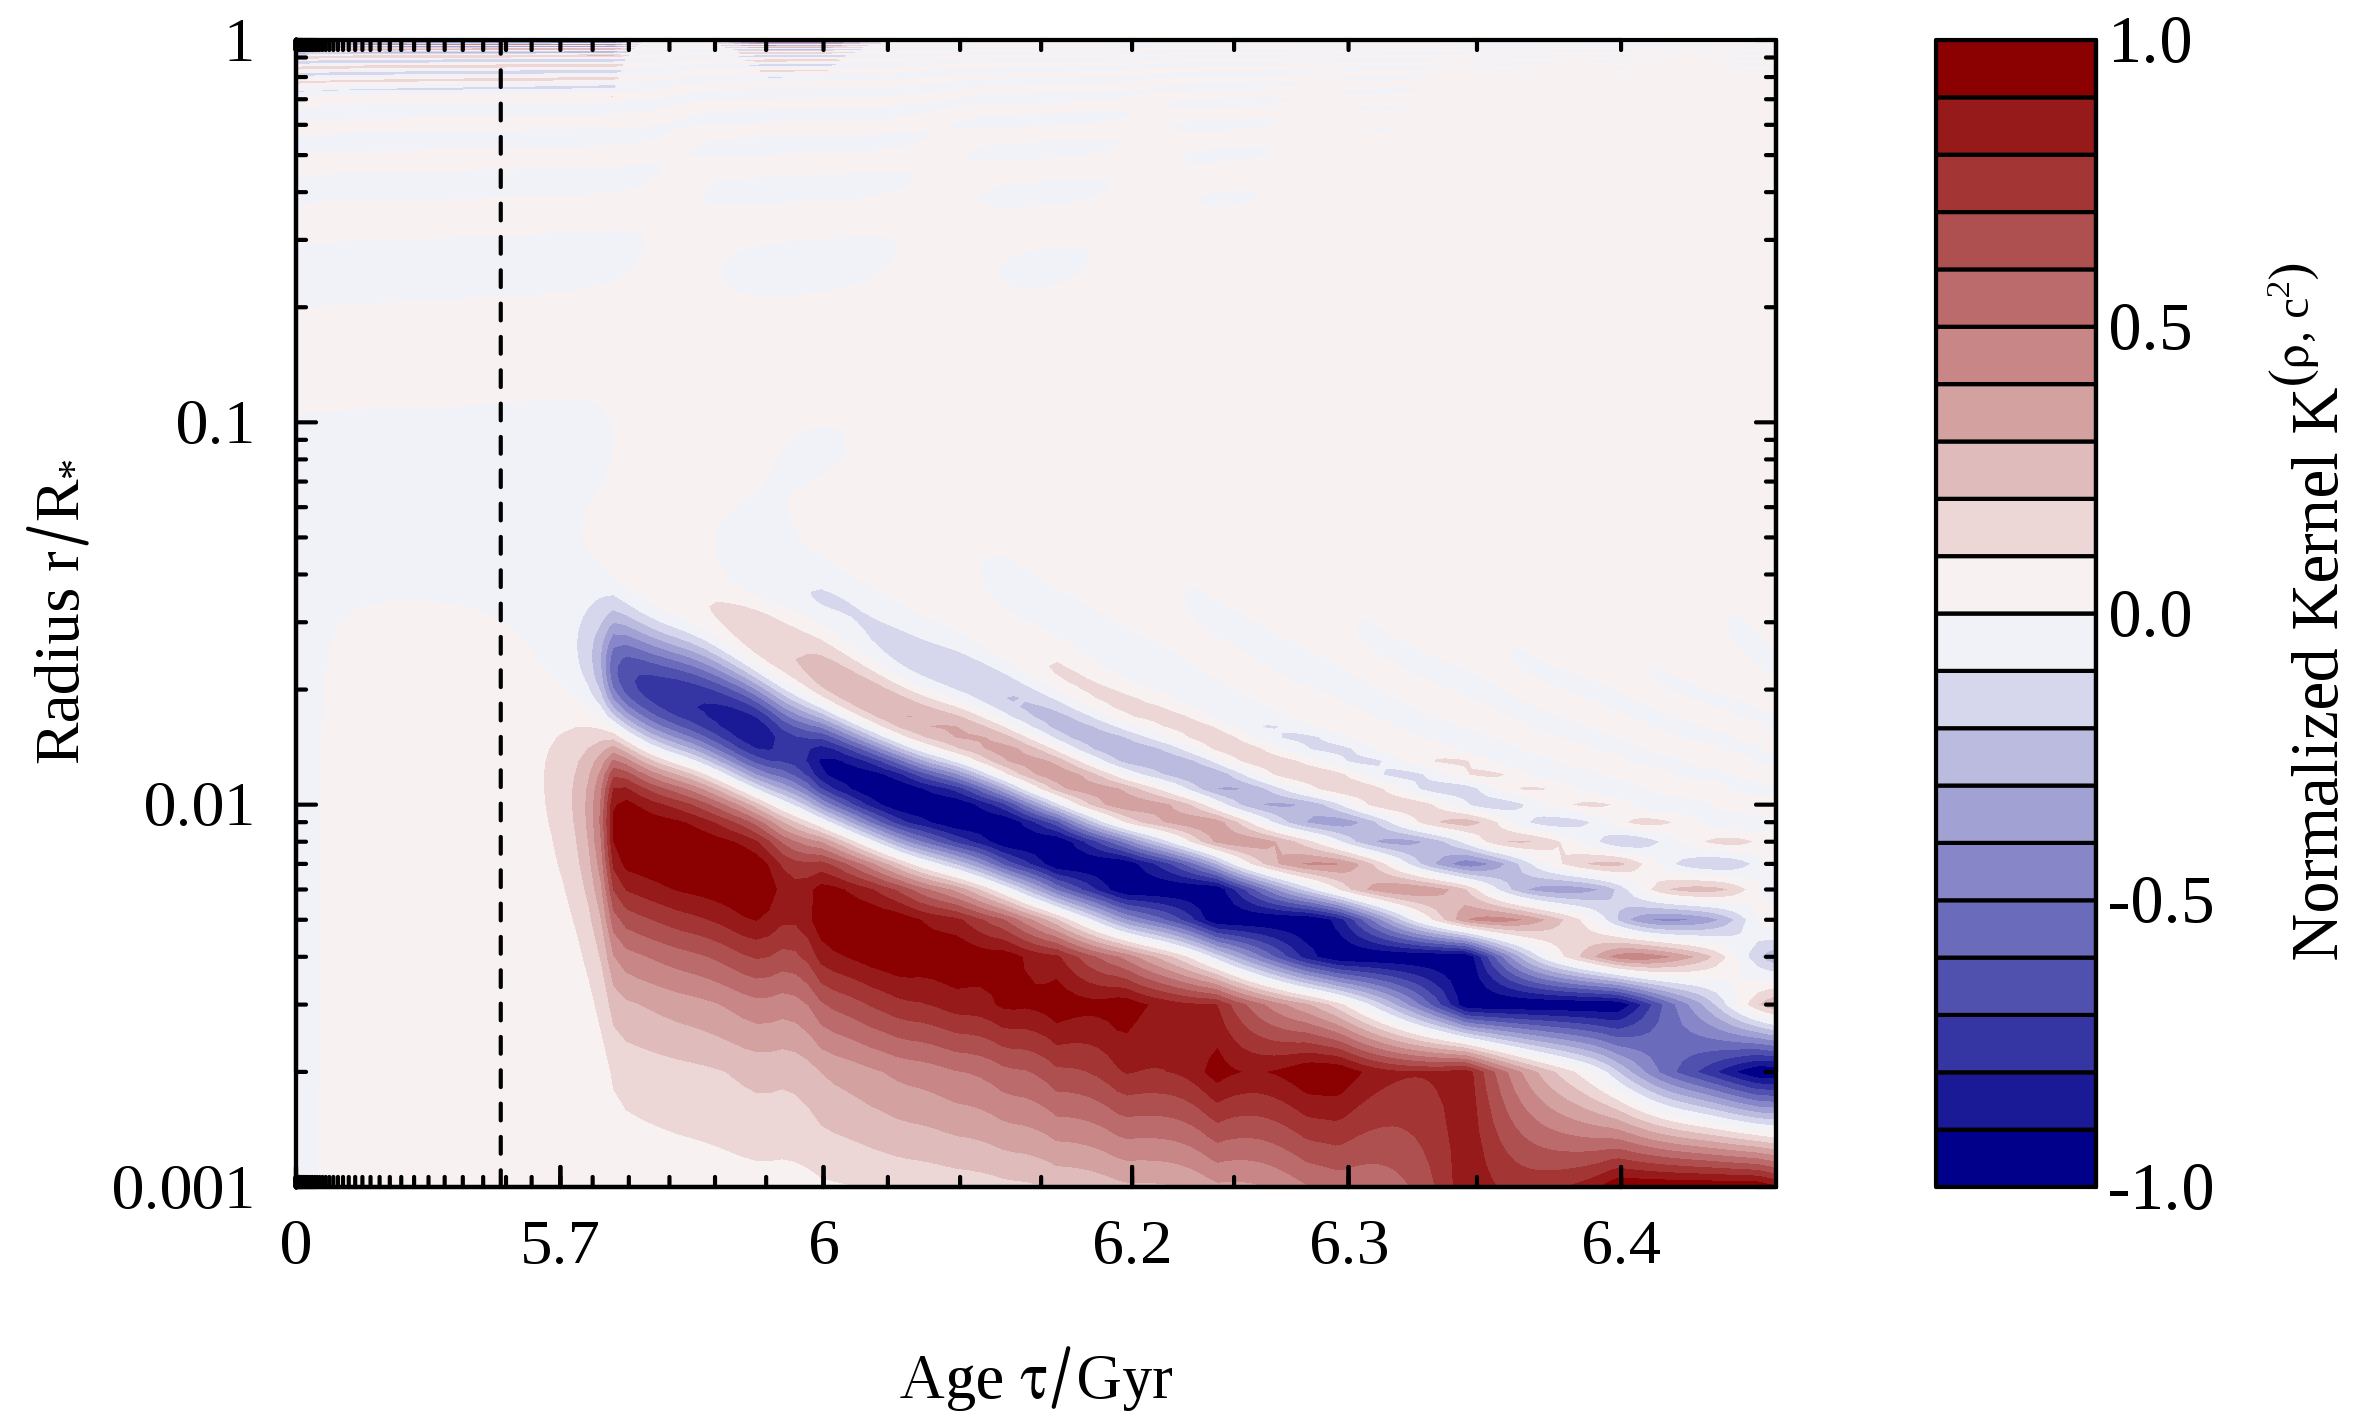
\includegraphics[width=1.2\linewidth]{ch1_introduction/figs/prospective/kernel_evolution-rho-c2-l1_n11.png}
    \caption[Kernel function evolution]{Evolution of the (${\rho, c^2}$) kernel function for the (${\ell=1}, {n=11}$) mode of a ${1.11\; M/M_\odot}$ star. 
        The vertical dashed line shows the end of the main sequence (TAMS). 
        As the mode mixes with a $g$-mode, it develops extreme sensitivity to the deep core structure of the star. 
        \label{fig:kernel-evol}}
\end{figure}
%\end{landscape}
    
    
    \item[Evolution inversions for fundamental constants.]
    A problem of cosmological significance is the measurement of physical constants, and the determination of whether or not they really are constant. 
    The idea of using the Sun to constrain the cosmic variation of the gravitational constant $G$ goes back at least to the time of \citet{Dirac199}. 
    So far, this approach has not been undertaken using other stars. 
    I intend to use the tools discussed in this thesis to measure $G$ as well as other fundamental quantities that impact on stellar evolution and pulsation, such as the fine structure constant \citep[e.g.,][]{2008JCAP...08..010A, 2010AIPC.1269...21C}. 
    Though the Sun is the star with the best data, observations of a large number stars may be able to be combined into a more sensitive tool for these measurements. 
    Furthermore, the Sun's evolution only covers one third of the history of the Universe, and is therefore insensitive to any earlier variations to these quantities. 
\end{description}

In the longer term, there are other prospects that are quite exciting. 
\citet{2014ApJ...782....2L} predicted that $\ell=4$ modes would be observable in 16~Cyg~A and B from \emph{Kepler} data. 
With such data, it would be possible to resolve the sound speed profiles of the observed stars to even shallower layers, which would provide further constraints on theories of the stellar interior. 
However, recent data releases seem not to have produced any such detections. 
%It does not seem that this was the case. 
It does seem feasible within the coming decades that such observations could become available, perhaps through a combination of \emph{Kepler} data with SONG observations \citep{2014RMxAC..45...83A, 2017ApJ...836..142G} and possibly utilizing the forthcoming TESS and PLATO missions. 

In this thesis, I used artificial intelligence to assist in solving problems in stellar astrophysics. 
This is a form of so-called \emph{weak} AI. 
These tools will only get more powerful with the coming decades. 
Eventually, we may have \emph{strong} AI, which will be capable of fully driving scientific research. 
One day, it may be that AI will be able to determine on its own the set of astrophysical laws that are most harmonious with enormous quantities of empirical data. 

%Eventually, I foresee the possibility of AI fully driving scientific research, determining on its own the set of physical laws that are most consonant with enormous quantities of data. 

%In the even longer term, 
%inversions of subgiants 
%inversions of red giants 
%ML of sub and red giants 
%diagnostics from nonradial modes of evolved stars 
%galactic archaeology 
%stars as laboratories to find fundamental constants 
%observations of high degree modes in other stars 
%AI-driven discovery of natural laws 
%\subsection*{Short-Term Prospects}
%\subsection*{Long-Term Prospects}
